\chapter{Regression}
\newcommand{\linkAutoSklearnRegressor}{https://automl.github.io/auto-sklearn/master/examples/20_basic/example_regression.html}

Within auto-sklearn, we can make use of the \href{\linkAutoSklearnRegressor}{'AutoSklearnRegressor'\footnote{AutoSklearnRegressor: \href{\linkAutoSklearnRegressor}{\linkAutoSklearnRegressor}}} to implement a model for a regression problem.

\section{Used Car Prices}
\newcommand{\kagglelinkusedcaruk}{https://www.kaggle.com/adityadesai13/used-car-dataset-ford-and-mercedes?select=vw.csv}

For this dataset we used the competition version of a big data set provided on  This set is based on a big \href{\kagglelinkusedcaruk}{dataset\footnote{Used Car UK:\href{\kagglelinkusedcaruk}{\kagglelinkusedcaruk}}} of 100 000 listings on used cars in the UK. We then found and used a version that was slimmed down for competition. This dataset looked ideal for us to learn more about auto-sklearn.

\subsection{Dataset}
\newcommand{\kagglelinkusedcar}{https://www.kaggle.com/kukuroo3/used-car-price-dataset-competition-format}

The \href{\kagglelinkusedcar}{dataset\footnote{Used Car price Prediction:\href{\kagglelinkusedcar}{\kagglelinkusedcar}}} can be found on Kaggle and contains 12 features which can be used to predict price of used cars in the UK. Those features are:

\begin{itemize}
    \item carID: The id of the car in the dataset.
    \item brand: brand of the car.
    \item model year: Build year of the model.
    \item transmission: type of transmission.
    \item mileage: Total amount of mileage on the car.
    \item fuelType: Type of fuel.
    \item tax: Amount of tax.
    \item mpg: miles-per-gallon.
    \item engineSize: Size of the engine.
    \item price: price of the car.
\end{itemize}

\noindent There are 2672 observations in the dataset. For none of the features data is missing.

\subsection{Model Performance}

First we visualised the dataset with 2 different pairplots.
This gave us an idea of what to expected from this dataset.
The pairplot that is based on the fueltype shows clearly that petrol cars are the most common.
\begin{figure}
    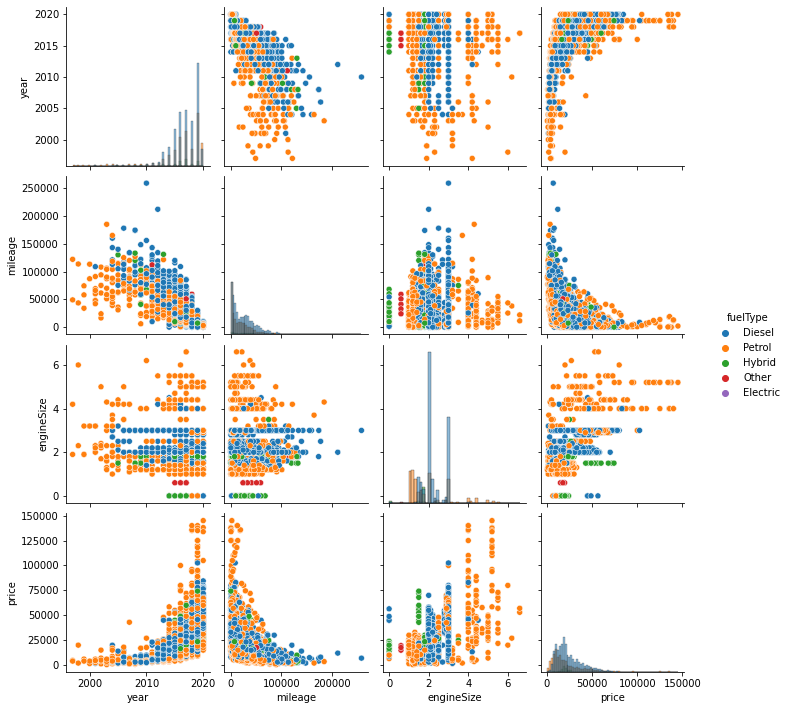
\includegraphics[width=\linewidth]{images/pairplot_fueltype.png}
    \caption{A pairplot based on fueltype}
    \label{fig:pairplot fueltype}
\end{figure}
The pairplot that is based on the brand shows clearly that the german brands are most common.
\begin{figure}
    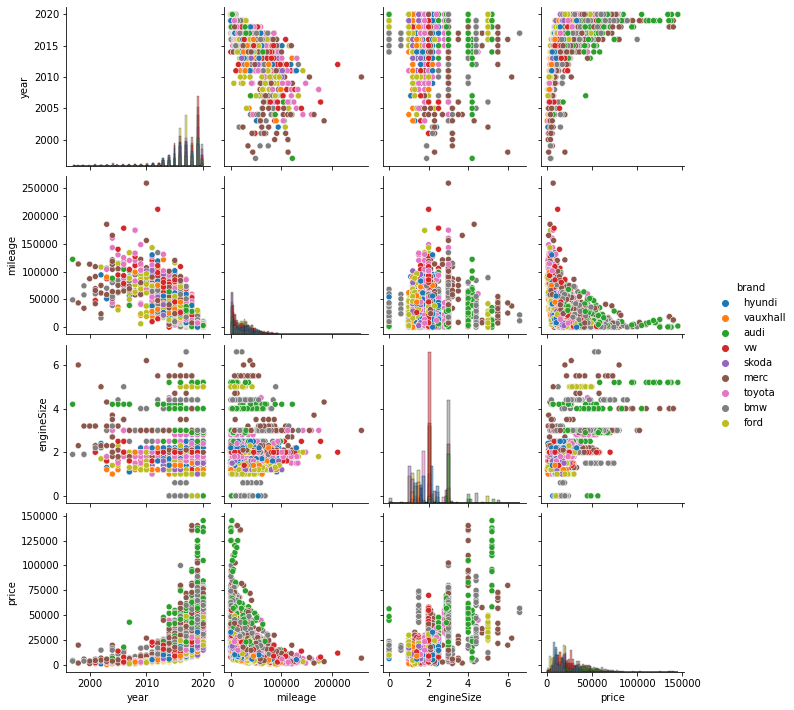
\includegraphics[width=\linewidth]{images/pairplot_brand.png}
    \caption{A pairplot based on brand}
    \label{fig:pairplot brand}
\end{figure}
\\
After fitting and training the data this are the results we got for the different data sets.

\begin{table}[h!]
    \begin{center}
        \caption{Table with training results.}
        \label{tab:training results}
        \begin{tabular}{l|S|r|l} % <-- Changed to S here.
            \textbf{function} & \textbf{Training data} & \textbf{Test data} & \textbf{Validation data}\\
            \hline
            mean squared error & 59050.4794 & 293230.5317 & 585230.4846\\
            mean absolute error & 26.3980 & 55.7094 & 59.8129\\
            r2 & 0.9998 & 0.9989 & 0.9979\\
        \end{tabular}
    \end{center}
\end{table}

\subsection{Model Comparision}
\newcommand{\kagglelinkusedcarcompare1}{https://www.kaggle.com/selinsong/u-car-rf-r2-score-0-94/data}
\newcommand{\kagglelinkusedcarcompare2}{https://www.kaggle.com/yuyuyuyuy/rf-test-r2-score-0-956}
\newcommand{\kagglelinkusedcarcompare3}{https://www.kaggle.com/johyunkang/py-rf-test-r2-0-939}
We chose 3 models from kaggle to compare our results with. After comparing our scores we found out that we have a better performing model. Our model included te model of the car, this was something the other models left out. We can conclude that our models performs better than the ones we compared scores with. We reference the chose models as \href{\kagglelinkusedcarcompare1}{Url1\footnote{Url1:\href{\kagglelinkusedcarcompare1}{\kagglelinkusedcarcompare1}}}, \href{\kagglelinkusedcarcompare2}{Url2\footnote{Url2:\href{\kagglelinkusedcarcompare2}{\kagglelinkusedcarcompare2}}} and \href{\kagglelinkusedcarcompare3}{Url3\footnote{Url3:\href{\kagglelinkusedcarcompare3}{\kagglelinkusedcarcompare3}}} in the table.

\begin{table}[h!]
    \begin{center}
        \caption{Table with r2 results.}
        \label{tab:training results}
        \begin{tabular}{l|S} % <-- Changed to S here.
            \textbf{data} & \textbf{R2 score} \\
            \hline
            Training data & 0.9997784238195022\\
            Test data & 0.9989334899119373 \\
            Validation data & 0.9978756073515518\\
            Url1 & 0.94\\
            Url2 & 0.956\\
            Url3 & 0.939\\
        \end{tabular}
    \end{center}
\end{table}

\section{Television Brand E-commerce}
This dataset can be used to explore the current market scenario for Televisions. There are various types of screens with different operating systems offered by several manufacturers at competitive prices.

\subsection{Dataset}
\newcommand{\kagglelinktv}{https://www.kaggle.com/devsubhash/television-brands-ecommerce-dataset}

This \href{\kagglelinktv}{dataset\footnote{Television dataset:\href{\kagglelinktv}{\kagglelinktv}}} includes specifications of different televisions offered by various brands with prices and ratings.
It contains 912 samples with 7 attributes. Here are the columns in this dataset-
Brand Resolution Size Selling Price Original Price Operating System Rating

\begin{itemize}
    \item Brand: This indicates the manufacturer of the product i.e. Television
    \item Resolution: This has multiple categories and indicates the type of display i.e. LED, HD LED, etc.
    \item Size: This indicates the screen size in inches
    \item Selling Price: This column has the Selling Price or the Discounted Price of the product
    \item Original Price: This includes the Original Price of the product from the manufacturer.
    \item Operating system: This categorical variable shows the type of OS like Android, Linux, etc.
    \item Rating: Average customer ratings on a scale of 5
\end{itemize}

\subsection{Model Performance}
First we visualised the dataset with a pairplot.
This gave us an idea of what to expected from this dataset.
The pairplot that is based on the resolution shows clearly HD LED and ULTRA HD LED are the most common resolution.
\begin{figure}
    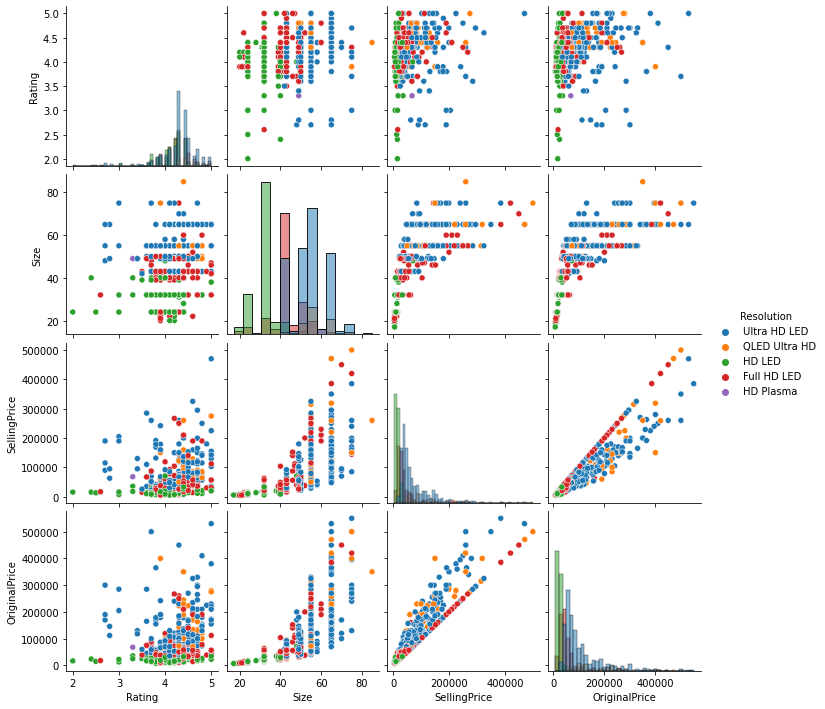
\includegraphics[width=\linewidth]{images/pairplot_resolution.png}
    \caption{A pairplot based on tv resolution}
    \label{fig:pairplot resolution}
\end{figure}

After fitting and training the data this are the results we got for the different data sets.

\begin{table}[htp]
    \begin{center}
        \caption{Table with training results.}
        \label{tab:training results}
        \begin{tabular}{l|S|r} % <-- Changed to S here.
            \textbf{function} & \textbf{Training data} & \textbf{Test data} \\
            \hline
            mean squared error & 81016219.59417547 & 952681194.3707451 \\
            mean absolute error & 5251.913730638445 & 14205.972881317139 \\
            r2 & 0.9796709758590545 & 0.8247644898857763\\
        \end{tabular}
    \end{center}
\end{table}

\subsection{Model Comparision}
\newcommand{\kagglelinktvcode}{https://www.kaggle.com/devsubhash/television-brands-ecommerce-dataset/code}

When we looked on the \href{\kagglelinktvcode}{kaggle\footnote{Television code page:\href{\kagglelinktvcode}{\kagglelinktvcode}}} page of this dataset we found out that there are not yet any other auto-sklearn projects submitted. Thats why we can not compare our results with someone else. We do notice te big difference between test and training data results.
